\chapter*{Findings}
\begin{table}[htb]
    \renewcommand{\arraystretch}{1.5}
    \begin{tabular*}{\textwidth}{|>{\columncolor{orange!15}}p{3cm}|p{17.1cm}|}
    \textbf{Finding} & \textbf{Coding mistake leads to disk-image access}\\
    
	&\\
	Description& By analyzing the processes of the server we found that a compiled python file 'fdesetup.pyc' is executed directly after rebooting the server. Unfortunately it is not possible to read a compiled python file without decompiling it. The contents of the 'fdesetup.pyc' file appear as follows:
    \newline
    \newline
    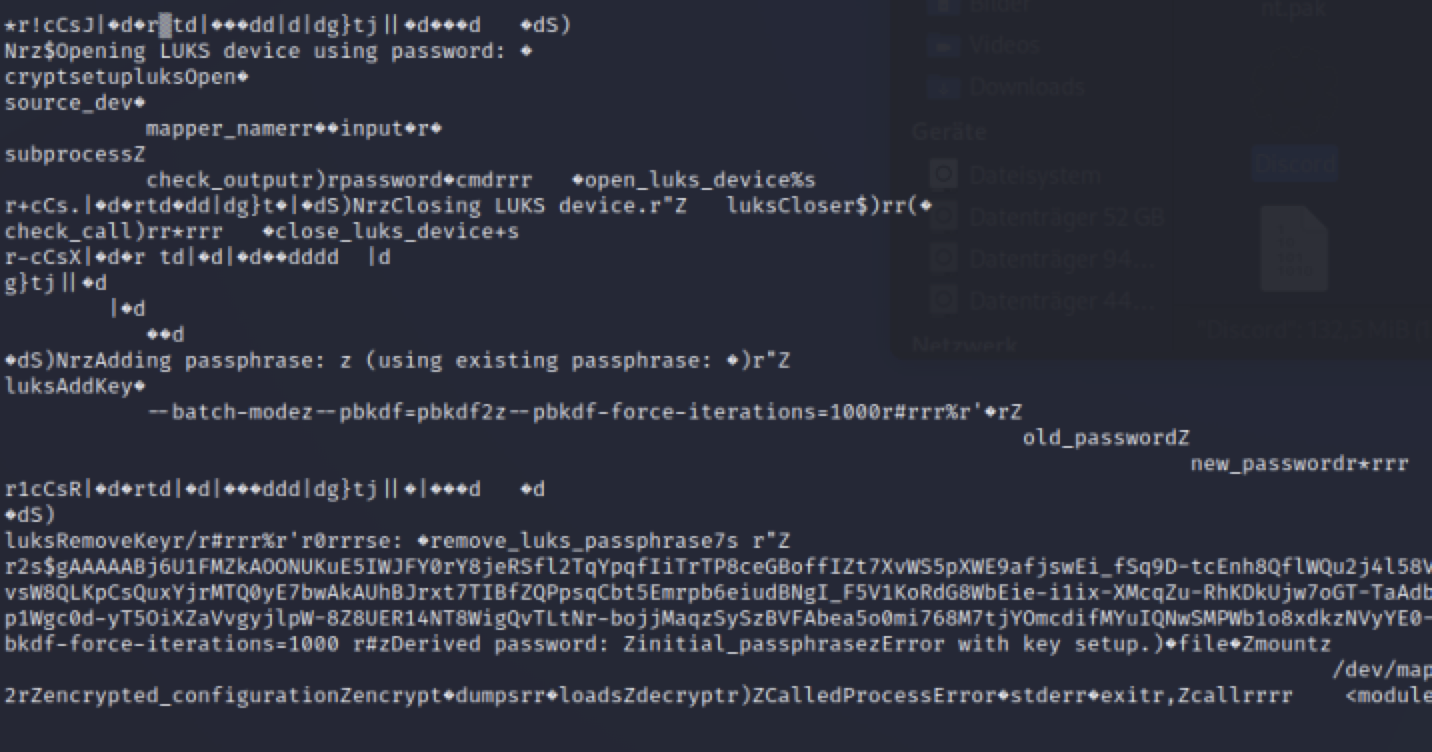
\includegraphics[width=0.73\textwidth]{fdesetup_pyc.png}
    \newline 
    \newline
    The few readable keywords inside the file like 'passphrase' or 'cryptsetupluksOpen' indicate that it must be a configuration for the 'cryptsetup luks' libary. 
    Therefore the file was copied to the local kali machine to decompile it. 
    \\
	&\\
    Recommendation&\\    
    \end{tabular*}
    \end{table}